\documentclass{article}
\setlength{\parskip}{0pt} % esp. entre parrafos
\setlength{\parindent}{20pt} % esp. al inicio de un parrafo
\usepackage{amsmath} % mates
\usepackage{listings}
\usepackage[sort&compress,numbers]{natbib} % referencias
\usepackage{url} % que las URLs se vean lindos
\usepackage[top=10mm,left=20mm,right=20mm,bottom=25mm]{geometry} % \textbf{\textbf{}}margenes
\usepackage{hyperref} % ligas de URLs
\usepackage{graphicx} % poner figuras
\usepackage[spanish]{babel} % otros idiomas
\hypersetup{
    colorlinks=true,
    linkcolor=blue,
    filecolor=blue,      
    urlcolor=blue,
}

\title{Reporte 1:\\Movimiento Browniano}
\author{1642654 Jorge Alejandro Torres Quintanilla}
\date{\today}

\begin{document}

\maketitle

\section{Objetivo}
Esta pr\'actica tiene como objetivo el estudiar de manera sistem\'atica el movimiento aleatorio de una part\'icula en un espacio que va de 1 a 5 dimensiones. Se var\'ia tambi\'en la cantidad de pasos que dura la caminata, y para cada caminata en cada dimensi\'on, el experimento se repite 30 veces. Los resultados se observan un una sola gr\'afica con diagramas caja-bigote. Asimismo, se eval\'ua el tiempo promedio en que se realiza el c\'omputo de una r\'eplica del experimento.

\section{Desarrollo}
En mi \href{https://github.com/FeroxDeitas/Simulacion-Nano/tree/main/Tareas/P1}{repositorio} de GitHub se puede observar la evoluci\'on del c\'odigo desarrollado. Tomando como base el \href{https://github.com/satuelisa/Simulation/blob/master/BrownianMotion/sinpar.py}{c\'odigo} proporcionado por la Dra. Elisa Schaeffer \cite{elisa1}, se hace una modificaci\'on para iterar entre la cantidad de pasos que se realizan en cada dimensi\'on. A continuaci\'on el c\'odigo utilizado para la pr\'actica.

\begin{lstlisting}

from random import random, randint
from math import sqrt
import matplotlib.pyplot as plt
import numpy as np
from time import time

runs = 30 #replicas
caminatas = [100, 1000, 10000] #pasos
results = [] #almacena las dimensiones

for i in range(3): #itera la cantidad de pasos
    dur = caminatas[i]
    for dim in range(1, 6): #de una a cinco dimensiones
        mayores = []
        for rep in range(runs):#corre el experimento 30 veces en cada dimension
            before = time()*1000
            pos = [0] * dim
            mayor = 0
            for paso in range(dur):
                eje = randint(0, dim - 1)
                if pos[eje] > -100 and pos[eje] < 100:
                    if random() < 0.5:
                        pos[eje] += 1
                    else:
                        pos[eje] -= 1
                else:
                    if pos[eje] == -100:
                        pos[eje] += 1
                    if pos[eje] == 100:
                    pos[eje] -= 1
                mayor = max(mayor, sqrt(sum([p**2 for p in pos])))
                after = time()*1000
            mayores.append(mayor)
        results.append(mayores)
tiempo = after - before
print(tiempo)

#separar los resultados en tres grupos de caminatas
walks_1 = results[0:5] #caminatas de 100 pasos
walks_2 = results[5:10] #caminatas de 1000 pasos
walks_3 = results[10:15] #caminatas de 10000 pasos

#empezar a graficar

ticks = ['1', '2', '3', '4', '5']

#funcion definir los colores de cajas y bigotes
def set_box_color(bp, color):
    plt.setp(bp['boxes'], color=color)
    plt.setp(bp['whiskers'], color=color)
    plt.setp(bp['caps'], color=color)
    plt.setp(bp['medians'], color='orange')

plt.figure()

bpl = plt.boxplot(walks_1, positions=np.array(range(len(walks_1)))*5.0-1.0, \
                  sym='', widths=0.8)
bpc = plt.boxplot(walks_2, positions=np.array(range(len(walks_2)))*5.0, \
                  sym='', widths=0.8)
bpr = plt.boxplot(walks_3, positions=np.array(range(len(walks_3)))*5.0+1.0, \
                  sym='', widths=0.8)
set_box_color(bpl, '#D7191C')
set_box_color(bpc, '#2CB62C')
set_box_color(bpr, '#2C7BB6')

#leyenda
plt.plot([], c='#D7191C', label='100 pasos')
plt.plot([], c='#2CB62C', label='1000 pasos')
plt.plot([], c='#2C7BB6', label='10000 pasos')
plt.legend()

plt.xticks(range(0, len(ticks)*5, 5), ticks)
plt.xlim(-2, len(ticks)*5)
plt.title('Distancia Euclideana')
plt.xlabel('Dimensiones')
plt.ylabel('Distancia Maxima')
plt.tight_layout()
plt.savefig('DistanciaEucl.png')
plt.show()
\end{lstlisting}

Como se observa, primero se realizan 30 ciclos de 100 pasos en una a cinco dimensiones, despu\'es con 1,000 pasos y por \'ultimo con 10,000 pasos. En cada ciclo se calcula la distancia m\'axima euclideana tomada desde el punto de origen utilizando la ecuaci\'on \eqref{eq1} y se agrega a la lista de resultados para ser graficados posteriormente.

\newpage

\begin{equation}
    d_{max} = \sqrt{\sum_{n=1}^m x_{n}^{2}}\\ \label{eq1}
\end{equation}
Donde $m$ es la cantidad de ejes.\\

Adicionalmente, se utiliza el comando \texttt{time()} para medir el tiempo que toma realizar los 30 ciclos en cada dimensi\'on, a lo cual se realiza una normalizaci\'on para conocer el promedio que tarda en ejecutarse un solo ciclo.

\section{Resultados}

\subsection{Distancia M\'axima Euclideana}
En la figura \ref{figura1} se puede observar la agrupaci\'on estad\'istica de las distancias m\'aximas recorridas por una part\'icula con movimiento aleatorio al realizar caminatas de 100 (rojo), 1,000 (verde) y 10,000 (azul) pasos, para espacios cartesianos con 1 a 5 ejes. Cabe resaltar que estos ejes tienen un rango de -100 a 100 unidades, y que la part\'icula retrocede un paso al llegar al borde.

\begin{figure}[h]
    \centering
    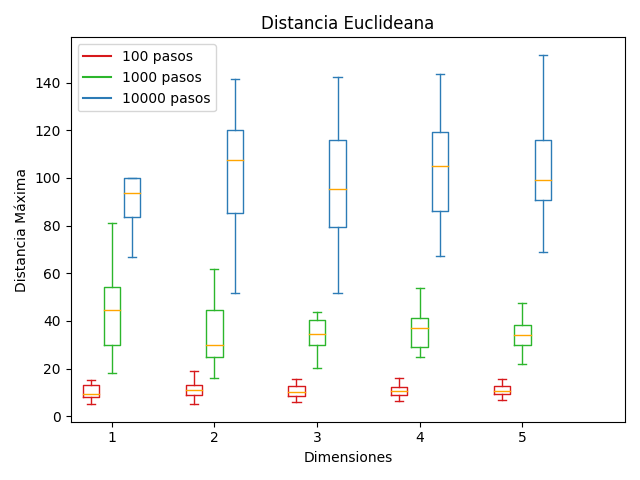
\includegraphics[width=150mm]{DistanciaEucl.png}
    \caption{Diagrama caja-bigote donde se observan las estad\'isticas de distancia m\'axima euclideana para los grupos de 100, 1,000 y 10,000 pasos en dimensiones de 1 a 5.}
    \label{figura1}
\end{figure}

\newpage

\subsection{Tiempo de Ejecuci\'on}
Al realizar un estudio automatizado del tiempo que tarda una repetici\'on en ejecutarse y calcular un promedio al correr el programa varias veces, se puede crear una idea aproximada de lo eficiente que es el c\'odigo para la tarea en cuesti\'on. Los resultados de tal estudio se muestran en el cuadro \ref{cuadro1} y se puede observar que mi computadora tarda $\approx$ 32 ms en completar una repetici\'on de 30 ciclos del experimento, por lo que se estima que tardar\'ia $\approx$ 1.06 ms en completar un ciclo.

\begin{table}
    \centering
    \caption{Tiempo promedio que tarda una repetici\'on de 30 ciclos en realizarse.}
    \begin{tabular}{|c|r|}
    \hline
        \textbf{Repetici\'on} & \textbf{Tiempo (ms)} \\
    \hline\hline
        1  & 31.2421875 \\
    \hline
        2 & 31.278564453125 \\
    \hline
        3 & 37.772216796875 \\
    \hline
        4 & 28.126953125 \\
    \hline
        5 & 31.248291015625 \\
    \hline
        6 & 31.731201171875 \\
    \hline
        7 & 31.338134765625 \\
    \hline
        8 & 31.368896484375 \\
    \hline
        9 & 31.35498046875 \\
    \hline
        10 & 33.336669921875 \\
    \hline
        \textbf{Promedio} & 31.8798085703125 \\
    \hline
    \end{tabular}
    \label{cuadro1}
\end{table}

\section{Conclusi\'on}
Al observar los diagramas de la figura \ref{figura1} se puede apreciar c\'omo el rango de distancia m\'axima es cada vez m\'as amplio al aumentar la cantidad de pasos, lo cual se debe a que tiene m\'as posibilidades de terminar en puntos diferentes del espacio. Por otro lado, el rango de distancias no aumenta o disminuye significativamente al variar la cantidad de ejes en que se puede mover la part\'icula.\\

Tomando en cuenta que el tiempo promedio de ejecuci\'on de una repetici\'on es de 32 ms y que se realizan 15 repeticiones (5 grupos de dimensiones por 3 grupos de largo de caminata), se tiene que el programa deber\'ia tardar $\approx$ 480 ms en ejecutarse. La realidad es que tarda m\'as debido a que debe realizar y guardar la gr\'afica en un archivo PNG. Adem\'as, existe la posibilidad de paralelizar operaciones al reservar n\'ucleos del CPU para ejecutar el programa, lo cual no se ha implementado en esta ocasi\'on.

\bibliography{tarea1}
\bibliographystyle{plainnat}
\end{document}
